\documentclass{standalone}
\usepackage{tikz}
\begin{document}
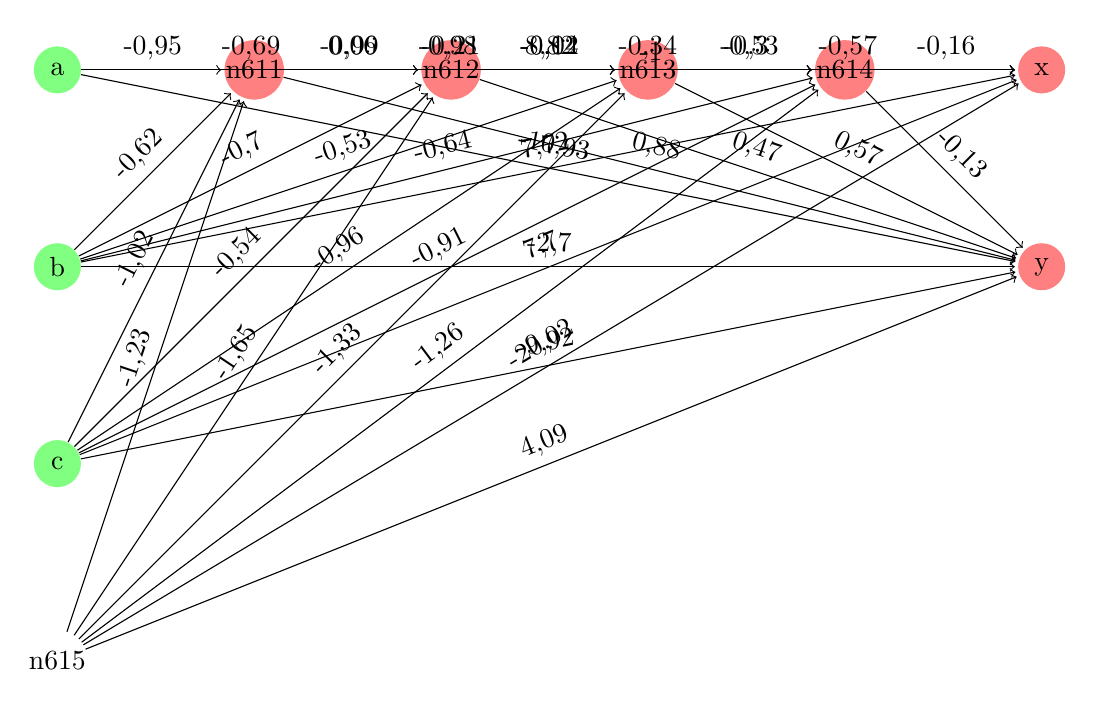
\begin{tikzpicture}[shorten >=1pt,->,draw=black!,node distance=2.5cm]
\tikzstyle{neuron}=[circle,fill=black!25,minimum size=17pt,inner sep=0pt]
\tikzstyle{constant}=[neuron, fill=white!50];
\tikzstyle{identity}=[neuron, fill=green!50];
\tikzstyle{sigmoid}=[neuron, fill=red!50];
\node [identity] (a) {a};
\node [identity,below of=a] (b) {b};
\node [identity,below of=b] (c) {c};
\node [constant,below of=c] (n615) {n615};
\node [sigmoid,right of=a] (n611) {n611};
\node [sigmoid,right of=n611] (n612) {n612};
\node [sigmoid,right of=n612] (n613) {n613};
\node [sigmoid,right of=n613] (n614) {n614};
\node [sigmoid,right of=n614] (x) {x};
\node [sigmoid,below of=x] (y) {y};
\path[every node/.style={sloped,anchor=south,auto=false}]
(b) edge node {-2,7} (y)
(b) edge node {7,72} (x)
(b) edge node {-0,64} (n614)
(b) edge node {-0,53} (n613)
(b) edge node {-0,7} (n612)
(b) edge node {-0,62} (n611)
(a) edge node {8,82} (x)
(a) edge node {-0,99} (n613)
(a) edge node {-0,69} (n612)
(a) edge node {-0,95} (n611)
(a) edge node {-10,93} (y)
(a) edge node {-0,98} (n614)
(c) edge node {-1,02} (n611)
(c) edge node {-9,92} (y)
(c) edge node {7,7} (x)
(c) edge node {-0,91} (n614)
(c) edge node {-0,96} (n613)
(c) edge node {-0,54} (n612)
(n612) edge node {-0,53} (x)
(n612) edge node {0,47} (y)
(n612) edge node {-0,12} (n613)
(n612) edge node {-0,34} (n614)
(n611) edge node {-1} (x)
(n611) edge node {0,88} (y)
(n611) edge node {0,06} (n612)
(n611) edge node {-0,21} (n613)
(n611) edge node {-0,04} (n614)
(n614) edge node {-0,16} (x)
(n614) edge node {-0,13} (y)
(n613) edge node {-0,57} (x)
(n613) edge node {0,57} (y)
(n613) edge node {-0,3} (n614)
(n615) edge node {-20,02} (x)
(n615) edge node {4,09} (y)
(n615) edge node {-1,23} (n611)
(n615) edge node {-1,65} (n612)
(n615) edge node {-1,33} (n613)
(n615) edge node {-1,26} (n614)
;\end{tikzpicture}
\end{document}